%   Titre de la sous sections
\section{Déterminer une vitesse avec \mbot}

%   logo mb ou st dans la table des matières
%\logo{mb}
\logo{mbot}
%\logo{st}

%
%   style de la page
%   commenter avec % le style non utilisé
%\pagestyle{mb} %pour microbit
\pagestyle{mbot} %pour mbot
%\pagestyle{st} %pour ST

\subsection{Description}

\subsubsection{Objectif}


%   bloc de formule
%   sans titre et fond bleu cyan
\begin{formule}
Le but de ce projet, liées au programme de Maths-Sciences en CAP ou Bac Pro, est d'utiliser le robot \mbot pour travailler sur le \textbf{mouvement} et la \textbf{mesure}.

Outre la \textbf{vitesse}, qui est au centre du projet, une travail sur l'\textbf{erreur}, l'\textbf{incertitude} et les \textbf{statistique} est possible.
\end{formule}


\subsubsection{Intérêt}

%liste d'arguments
\begin{description}
	\item [Détermination de mesures physiques] Ces activités proposent d'étudier un questionnement essentiel de physique : \emph{comment mesurer une vitesse} ? Deux grandeurs sont donc à déterminer le plus précisément possible : une \emph{distance} et un \emph{temps}.
	\item[Mouvement uniforme ou accéléré] Le robot \mbot met un certain temps à démarrer : le mouvement est donc accéléré puis uniforme. 
	\item [Travail sur l'incertitude]  
	Il est intéressant de déterminer la vitesse lorsque le \emph{mouvement est uniforme}. Ainsi il sera obligatoire de lancer le chrono après le départ. Ce qui est intéressant car cela engendre un travail sur l'\emph{erreur} et permet un calcul d'\emph{incertitude}.
	\item[Étude statistique] 	Un \emph{travail statistique} pourra découler de ces mesures. Par exemple, il est intéressant de déterminer de moyenne et écart type.
\end{description}


\subsubsection{Matériel}
\begin{itemize}
%   matériel pour MBot
\item 1 $\times$ \matosMbot
%   site internet pour MBot
   \item 1 $\times$ accès internet : IDE programmation par bloc \url{http://editor.makeblock.com/ide.html}
\end{itemize}



\subsubsection{Remarques}


%   bloc méthode
%   titre + fond bleu
\begin{methode}
    Dans la réalisation, nous suggérons d'utiliser un seul robot puis de demander aux élèves de mesurer temps et distance (donner 1 chronomètre par groupe ou utiliser les téléphone).\\
    Récupérer ensuite l'ensemble des résultats (une dizaine) puis proposer de les exploiter afin de déterminer une \emph{valeur précise et acceptable} de durée et distance. Il sera sans doute nécessaire de refaire les expériences au besoin.\\
	L'objectif n'est pas d'obtenir des valeurs identiques, mais d'\emph{analyser les conditions de l'expérience et de mesures} pour en améliorer la précision.
\end{methode}

%
% activité de niveau 
%

%   saut de page
\newpage

%   titre de la sous section
\subsection{Niveau initiation - Programmer le déplacement de \mbot}

\subsubsection{Activité élève}

% commande perso \CARTOUCHE
%   5 paramètres : 
%       * durée
%       * public
%       * travail en maths
%       * travail en sciences
%       * travail en algo
\cartouche
{1 h}         %durée
{2de}           %public
{translation}        %maths
{}     %sciences
{instructions de déplacement ; temporisation ; entrées clavier}       %algo


\begin{eleve}
Dans le cadre de la \href{https://www.youtube.com/watch?v=HMhzLhQLoBQ}{conduite autonome d’un véhicule} le conducteur programme la vitesse à laquelle il souhaite rouler.

\texttt{\large\textsc{Ta Mission} : Programmer le déplacement du robot MBot en utilisant le logiciel MBlock ?}
\end{eleve}


\begin{eleve}
\texttt{\large\textsc{Ta Mission} : Stopper le déplacement du robot MBot si l’on presse la touche « Espace » du clavier.}
\end{eleve}



\subsubsection{Notes pour l'enseignant}

\begin{minipage}[t]{0.5\linewidth}
    \begin{methode}~\\
        La plupart des élèves ne vont pas prévoir de stopper le robot.
        
        \centering{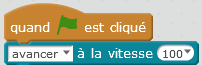
\includegraphics[width=0.5\linewidth]{res/mbot-vitesse-01.png}}
        
        Ils devront trouver comment modifier leur programme.
        
        \centering{
        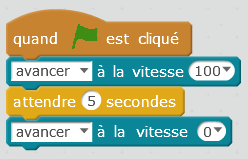
\includegraphics[width=0.45\linewidth]{res/mbot-vitesse-02.png}\hfill
        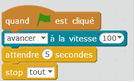
\includegraphics[width=0.45\linewidth]{res/mbot-vitesse-03.png}
        }
        
        
    \end{methode}
\end{minipage}
\hfill
\begin{minipage}[t]{0.5\linewidth}

    \begin{remarque}~\\
        
        Concernant la \emph{conduite autonome}, il est possible de montrer la première minute de \href{https://www.youtube.com/watch?v=HMhzLhQLoBQ}{cette vidéo}.
        
        
        Il est possible d'utiliser des \emph{vitesses différentes} que celles proposées ou encore des \emph{vitesse négatives}.
        
        \centering{
        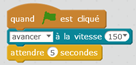
\includegraphics[width=0.45\linewidth]{res/mbot-vitesse-04.png}
        \hfill
        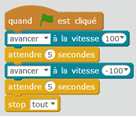
\includegraphics[width=0.45\linewidth]{res/mbot-vitesse-05.png}
        }
    \end{remarque}

\end{minipage}

\newpage
\subsection{Niveau intermédiaire - Déterminer la vitesse de \mbot}

\subsubsection{Activité élève}

% commande perso \CARTOUCHE
%   5 paramètres : 
%       * durée
%       * public
%       * travail en maths
%       * travail en sciences
%       * travail en algo
\cartouche
{1 h}         %durée
{2de}           %public
{conversions de grandeurs}        %maths
{mesure et incertitude ;  vitesse linéaire ; temps ; distance ; mouvement}     %sciences
{}       %algo


%   petite image de logo qui va
%   se mettre dans le bloc élève
\begin{wrapfigure}[4]{r}{4cm}
    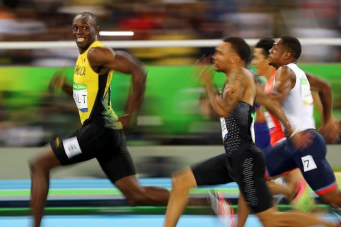
\includegraphics[width=\linewidth]{res/mbot-vitesse-sprint.png}
\end{wrapfigure}

%   bloc élève
%   fond orange
\begin{eleve}    

Karim et Julien programment le robot \mbot pour qu’il se déplace. Julien annonce à Karim :

\vspace{1em}

\begin{minipage}{0.65\linewidth}
    \emph{« Lorsqu’on sélectionne avancer à la vitesse 100 , cela ne correspond pas à 100 km/h mais à 100 m/s !!! »}
\end{minipage}

\vspace{1em}

\texttt{\Large\textsc{Ta Mission} : Comment vérifier l’\emph{affirmation} de Julien ?}
    
%   ajout d'une image
    %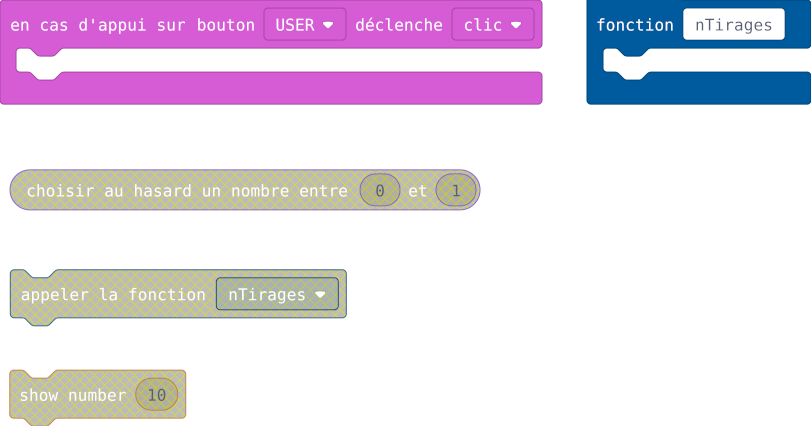
\includegraphics[width=0.5\linewidth]{res/st-pf-00-eleve.png}
\end{eleve}



\subsubsection{Notes pour l'enseignant}

%
%   méthode et remarque
%


\begin{minipage}[t]{0.5\linewidth}
    \begin{methode}~\\
        En général, les élèves utilisent leur programme du fichier « MBot1 », leur téléphone (pour mesurer le temps)
        et une règle (pour déterminer une distance). 
        
        La conversion des vitesses m/s et km/h est au centre de l’activité
        
        ~\\
        \begin{center}
            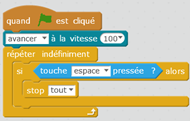
\includegraphics[width=0.85\linewidth]{res/mbot-vitesse-sol.png}
        \end{center}
    \end{methode}
\end{minipage}
\hfill
\begin{minipage}[t]{0.5\linewidth}
    \begin{remarque}~\\
        Très peu attendent que le robot ait déjà atteint une certaine vitesse avant de
        démarrer le chronomètre. Cela peut induire une réflexion sur le mouvement
        accéléré puis uniforme.
        
        %La proposition de solution \emph{interactive} est accessible en ligne \url{https://makecode.com/_EMYM0YfT11A6}.
    \end{remarque}

\end{minipage}